% Welcome to the unofficial template of the master study Smart Systems Engineering at Hanze University of Applied Sciences. Original template created by Natanael Magno Gomes and The Polytechnic Institute of Bragança (IPB).
% Adapted to Hanze's expectations by dr. Felipe Nascimento Martins and subsequently by Ewout Bergsma.
% All information of the "05_Final_report_format_20_21.docx" document is included in this template.
% Last update: 12/12/2021
% Feel free to contact me: ewoutbergsma [at] hotmail.com

\documentclass[12pt,a4paper,twoside]{ipb}
\errorcontextlines=3
\usepackage{csquotes}
\usepackage{amssymb}
\usepackage[portuguese,USenglish]{babel}
\graphicspath{{./images/}}
\usepackage{listings}
\usepackage{xcolor}
\usepackage{realboxes}
\usepackage{url}
\usepackage[colorlinks=true, urlcolor=black, linkcolor=black, citecolor=black, bookmarks=true, pdfstartview=FitH]{hyperref}

% \usepackage[style=ieee,backend=biber]{biblatex}
\usepackage[style=apa,backend=biber]{biblatex}
\addbibresource{references_field_removed.bib}
\usepackage{lipsum}
\usepackage{tabulary}
\usepackage{graphicx}
\usepackage{subfig}
\usepackage{float}  % Positioning of the figures
\usepackage[binary-units=true]{siunitx}
\usepackage[section]{placeins}
\usepackage{indentfirst}  % Indents all paragraphs
\usepackage{mathtools}  % Allows adding multi line equations
\emergencystretch=1em  % Fix overfull
\newcolumntype{P}[1]{>{\centering\arraybackslash}p{#1}}  % Centre col with width
\usepackage{enumitem}
\setlist{nosep}  % By default the separation is large
\renewcommand{\glsgroupskip}{}

\usepackage{adjustbox} % Include this in the preamble
% \usepackage{subcaption}

% \usepackage{subfigure}
\usepackage{subfig}



\usepackage{fancyref}  % This allows to use \fref{} command. This is very useful, it allows to easily refer to any \label{}. % See documentation: https://mirror.las.iastate.edu/tex-archive/macros/latex/contrib/fancyref/fancyref.pdf.
% \usepackage{cleveref} % Enhanced cross-referencing capabilities
% \usepackage{showframe}


\title{Counterfactual Analysis in Knowledge Graph Based Recommender System}  % Title of your thesis
\author{Celine Hovanessian Far}  % Student name
% \supervisor{Name First Supervisor}
% \cosupervisor{Name co-supervisor (Uncomment this line if there is no co-supervisor)}
% \courseyear{2024}
% \makeglossaries
% \loadglsentries{chapters/acronyms}


\begin{document}
\beforepreface  % Places thse cover page

\clearpage
% % Navigate to: chapters/abstract.tex
\begin{center}
    ABSTRACT
\vspace{5mm} %5mm vertical space
\end{center}

%%%%%%%%%%%%%%%%%%%%%%%%%%%%%%
Insert your abstract here. Original Hanze format states one can use a maximum of 200 words. Though, it is advised is to discuss with your supervisor(s) if you need more.
%%%%%%%%%%%%%%%%%%%%%%%%%%%%%%

\vspace{5mm} %5mm vertical space
\noindent {\bf Keywords:} Keyword, Keyword, Keyword.  % Replace keywords


\clearpage
% Navigate to: chapters/declaration.tex
% \begin{center}
    DECLARATION
    \vspace{5mm} %5mm vertical space
\end{center} 

I hereby certify that this report constitutes my own product, that where the language of others is set forth, quotation marks so indicate, and that appropriate credit is given where I have used the language, ideas, expressions or writings of another.

\vspace{1em}

I declare that the report describes original work that has not previously been presented for the award of any other degree of any institution.

\vspace{2em}

\noindent\hspace{8cm}Signed,
\begin{figure}[H]
    \hspace{8cm}
    
\includegraphics[width=6cm]{signature.png}  % Place an image of your signature in location: images/signature.png
    % Note how figures without \caption{} do not appear in the list of figures (same holds for tables)
\end{figure}

\noindent\hspace{8cm}Studentname Middlename Lastname  % Replace with your name


% \clearpage
% Navigate to: chapters/acknowledgements.tex
\begin{center}
    ACKNOWLEDGEMENTS
    \vspace{5mm} %5mm vertical space
\end{center} 

Here you have the opportunity to thank anyone. Acknowledgements should be in good taste and should not extend more than one page.  


\cleardoublepage  % Makes sure contents start on correct page
\afterpreface  % Places contents, list of tables and list of figures
\bodystart  % This sets stylistic parameters for the following content

% Here starts the actual content of your thesis
% \chapter{Rationale}\label{chap:rationale}
The first chapter of the Final Report should explain the rationale. It can be the same chapter as in your Master thesis definition, but you should incorporate any feedback that was given to you by your first graduation supervisor and your company supervisor \cite{jenelten2023dtc}.

% \chapter{Situational \& Theoretical Analysis}\label{chap:situational_theoretical_analysis}
This chapter in your final report can also be the same as in your master thesis definition, but should include all feedback that was given to you.
% \chapter{Conceptual Model}\label{chap:conceptual_model}

In this chapter you must explain, using the information from the previous two chapters and critical thinking, the most likely solution to your problem definition (narrowing down the theories and research), resulting in a final theory and/or model. Under a conceptual model it is understood that:  the author first investigates which factors play a role, and then provides argumentation for the identification of the most important ones. This chapter is basically a summary of chapter 2 and should be roughly 1 page long.



% \chapter{Research design}\label{chap:research}

The Research Design chapter contains everything that you have done in order to answer your research question. Write and state things in such a way that somebody can repeat your research and arrive at the exact same results. You can use the chapter in your master thesis definition as a start, but generally, research designs end up differently from what you intended to do in the first place. A special remark: it should be written in the PAST TENSE, since you now have already done it.


Note, the following content are some examples of techniques that one can use. Read the comments for explanations.


\section{Methodology}

A list of requirements has been defined to guide the project, a general and detailed design were developed and implemented to support the investigation of the research question.

\subsection{Requirements}

% One can replace \begin{enumerate} and \end{enumerate} with \begin{itemize} and \end{itemize} respectively for bullets instead of numbers.
\vspace{2mm}
\begin{enumerate}
  \item The Cobot safety features are enabled at all times.
  \item The system architecture is ROS based.
  \item The system works in simulation and real environment.
  \item The training is done using RL techniques.
  \item The algorithm is trained using self experience and memory replay.
  \item The algorithm uses RGBD images to estimate the actions.
\end{enumerate}
\vspace{3mm} 

\section{General Design}

General design text. See \fref{tab:models}.  % Note how \fref{} allows to refer to a label.

\section{Detailed Design}

Detailed design text. You don't have to follow this structure. Feel free to include, remove or change the titles of the sections.

An example of a table is shown in \fref{tab:models}. Moreover, an example of a figure is shown in \fref{fig:example_figure}. Always use the proper reference to cite tables and figures. Do not mention "table below" or "figure above", for example.

\begin{table}
    \centering
        \begin{tabular}{ p{35mm}  P{3cm}   P{40mm}  P{3cm}}
            \hline
            Model name & Feature space & Est. total size (MB) & Top-5 error \\
            \hline
            AlexNet          &   256  x 6 x  6     &  242.03  &    20.91 \\
            SqueezeNet       &   512  x 13 x 13   &   76.54   &    19.58 \\
            Densenet         &   1024 x 7 x  7    &   325.21  &    7.83  \\
            GoogleNet        &   1024 x 7 x  7    &   85.91   &    10.47 \\
            MobileNet        &   1280 x 7 x  7    &   162.45  &    9.71  \\
            ResNeXt-50-32x4d &   2048 x 7 x  7    &   415.72  &    6.30  \\
            MNASNet          &   1280 x 7 x  7    &   135.77  &    8.4  \\
            \hline
        \end{tabular}
    \caption{This is the caption of the example table \cite{torchvisionmodels}.}
    \label{tab:models}
\end{table}


\begin{figure}[b]  % b for bottom of page
    \centering
    
\includegraphics[width=0.8\textwidth]{images/hanzelogo_nl.png}
    \caption{This is the caption of the example figure.}
    \label{fig:example_figure}
\end{figure}



% \chapter{Research Results}\label{chap:research_results}

In the chapter discussing your research results you must provide all the results of your research in tables, graphs and figures format. Compare your results with the results found in literature or previous research and include all falsifications that you are aware of. Also comparisons must be made with the hypothesis you stated in the second chapter: are they correct? If so, why? If not, why not?
This chapter should include all the information that came out of your research and it should include a critical interpretation of these results.


% \chapter{Conclusions and Recommendations}\label{cap:conclusions_recommendations}

The last chapter contains the conclusions and recommendations. All your conclusions should be a logical consequence of the previous chapters that you have written and should provide answers to the research questions and problem definition posed in chapter \ref{chap:rationale}, \ref{chap:situational_theoretical_analysis} and \ref{chap:conceptual_model} 



% \chapter{Additional Chapters}\label{chap:additional_chapters}

If you want, you can add additional chapters to your final report. Keep in mind that the mentioned chapters should at least be present and the main text (excluding title page, table of contents, references and appendices) of the final report should not be more than 15000 words.

Note, if you need more words, please discuss with your supervisor(s).

1. Introduction to Counterfactual Analysis in Recommender Systems
•	Overview of Counterfactual Reasoning: Define counterfactual reasoning and its relevance in AI and recommender systems.
•	Importance in Explainability: Discuss the role of counterfactual analysis in enhancing the explainability of recommender systems.
1.B. XAI in KG Recommender Systems
The Knowledge-aware Path Recurrent Network (KPRN) addresses the challenge of enhancing both accuracy and explainability in recommender systems through the integration of knowledge graphs (KGs). KPRN exploits the rich connectivity information within KGs, using paths of entities and relations to deduce user preferences. It employs a Long Short-Term Memory (LSTM) network to process these paths, capturing the holistic semantics of user-item interactions. A weighted pooling mechanism is applied to prioritize significant paths, enhancing the model's predictive power and transparency. By doing so, KPRN significantly outperforms traditional methods, providing both improved recommendations and clear explanations of the reasoning behind these recommendations in real-world scenarios for movie and music recommendations. (Wang et al., 2019)

In the domain of explainable artificial intelligence (XAI) for knowledge graph (KG) recommender systems, the paper introduces an innovative approach called Path Language Modeling Recommendation (PLM-Rec). This framework leverages a path language model to dynamically predict and extend paths within a KG, allowing the recommendation system to reach previously unreachable items. By incorporating language modeling techniques, PLM-Rec overcomes traditional recall biases in KG-based recommenders, which are limited by the existing KG structure and a fixed number of hops. The technical novelty lies in training a language model on path sequences, akin to sentences in natural language, enabling the generation of new, plausible paths that expand the recommendation scope. This method integrates recommendation generation with explanations, offering transparent and intuitive paths that elucidate why items were recommended. Validated on multiple e-commerce datasets, PLM-Rec demonstrates superior performance in enhancing recommendation accuracy and addressing recall limitations compared to existing methods. (Geng et al., 2022)
This paper addresses the problem of enhancing recommendation accuracy and explanation personalization in recommender systems by integrating structured knowledge bases with collaborative filtering (CF). The proposed neural model leverages knowledge-base embeddings (KBE) to create a unified representation of user behaviors and item properties. It constructs a knowledge graph to encode these relationships and employs a soft matching algorithm for generating personalized explanations. Counterfactuals are generated by exploring different paths within the knowledge graph to determine the impact of various attributes on recommendations. Experimental results on real-world e-commerce datasets demonstrate improved accuracy and explainability, showcasing the model's effectiveness in providing meaningful and personalized recommendations. (Ai et al., 2018)

The paper "Cafe: Coarse-to-Fine Neural Symbolic Reasoning for Explainable Recommendation" addresses the challenge of improving recommendation performance and generating explanations in e-commerce recommender systems by incorporating knowledge graphs (KGs). Knowledge graphs provide rich, structured information about users and items, which can be leveraged to trace paths from users to recommended items, thereby offering explainable recommendations. However, the vast search space, unknown destinations, and sparse signals within the KG pose significant challenges. The Cafe approach tackles these issues with a two-stage process. In the coarse stage, user profiles are generated based on historical data, capturing prominent user behaviors. These profiles act as coarse sketches that guide the subsequent path-finding process. In the fine stage, these user profiles are used to direct a path-finding algorithm called Profile-guided Path Reasoning (PPR). This algorithm employs neural symbolic reasoning modules to efficiently and effectively discover recommendation paths within the KG. User profiles consist of patterns representing user behaviors, extracted from historical activity data. These profiles help focus the path-finding algorithm on relevant paths, improving both the efficiency and effectiveness of the recommendations. The experimental results, conducted on four real-world e-commerce datasets, show substantial improvements in recommendation performance compared to state-of-the-art methods. The paper highlights how integrating user profiles into the recommendation process provides better guidance for path reasoning, resulting in higher quality recommendations. The contributions of this paper include identifying shortcomings in previous KG reasoning approaches, particularly the separation of recommendation and path-finding tasks. Cafe introduces a new paradigm by explicitly incorporating diverse user behaviors into the KG reasoning process. The novel profile-guided path reasoning algorithm, utilizing neural symbolic reasoning modules, is empirically validated, showing significant performance gains across multiple benchmarks. In summary, the Cafe approach enhances e-commerce recommendation systems by integrating user behavior profiles with KG reasoning, enabling more accurate and explainable recommendations through an efficient path-finding process guided by neural symbolic reasoning. (Xian et al., 2020)

The paper addresses the challenge of making Graph Neural Networks (GNNs) explainable in the context of knowledge graphs (KGs). It introduces Monotonic GNNs (MGNNs), a novel class of GNNs that ensure transformations are explainable using logical rules in the Datalog formalism. The approach encodes KGs into graphs with numeric feature vectors, processes these graphs using MGNNs, and decodes the results back into KGs. MGNNs guarantee that transformations are equivalent to applying a set of Datalog rules, allowing for symbolic explanations. This method is applied to KG completion tasks, showing competitive performance while providing clear, logical explanations for predictions. The paper bridges the gap between machine learning and symbolic reasoning, enhancing interpretability in knowledge graph-based tasks. (Tena, et al, 2022)

The paper "Policy-Guided Path Reasoning (PGPR)" introduces a method to enhance the accuracy and explainability of recommendation systems using knowledge graphs (KGs) through explicit reasoning. Unlike traditional methods that primarily use KGs for accuracy, PGPR leverages them to provide interpretable recommendations. The approach employs reinforcement learning (RL), where an agent navigates the KG starting from a user node to find relevant items, offering reasoning paths that enhance interpretability. PGPR introduces innovative strategies such as a soft reward strategy, which designs rewards based on a multi-hop scoring function that accounts for heterogeneous information in the KG, and user-conditional action pruning to handle the large action space in KGs by pruning actions based on their relevance to the user, thereby reducing computational complexity. The policy-guided graph search algorithm efficiently samples reasoning paths during the recommendation process. The method was evaluated on several large-scale real-world datasets from Amazon, demonstrating superior performance compared to state-of-the-art methods using metrics like NDCG, Recall, Hit Rate, and Precision. By providing actual paths in the KG, PGPR makes the reasoning behind recommendations transparent and interpretable, addressing a critical need in modern recommendation systems. Overall, PGPR advances the field by coupling recommendation with interpretability, allowing users to understand the reasoning behind the system's suggestions. (Xian et al., 2019)

2. Counterfactual Methods in Different Types of Recommender Systems
•	Graph-based Recommender Systems: Focus on works like "Causal Inference for Knowledge Graph based Recommendation", highlighting how graph structures facilitate counterfactual reasoning.
•	Neural Recommender Systems: Explore studies such as "Counterfactual Explanations for Neural Recommenders", detailing methods specific to neural networks.
Counterfactual reasoning has been employed in recommender systems, serving a variety of purposes including bias reduction and enhancing explainability. By simulating conditions where certain variables are altered, counterfactual reasoning helps illuminate how such changes could affect outcomes, thereby offering insights into the underlying mechanics of recommender systems. This capability is crucial not only for refining system accuracy but also for ensuring the fairness and transparency of the recommendations provided.
In their study, Wei et al. (2023) introduce the KGCR model, an innovative approach designed to counteract bias in graph-based recommender systems by embedding causal inference within knowledge graph structures. This model enhances the accuracy of reflecting true user preferences through the use of Graph Convolutional Networks (GCNs) to refine the embeddings of users, items, and attributes. These enriched embeddings allow for more contextually informed representations. To mitigate biases, especially those originating from prior user interactions with specific attributes, the KGCR model constructs a causal graph. Interventions using do-calculus are applied to 'cut' edges representing biased influences, thereby creating counterfactual scenarios where such biases are excluded. This adjustment enables the recalibration of similarity scores, assessing potential outcomes had the user not engaged with the biasing attributes.

Further advancing the field, Tran et al. (2021) developed the ACCENT framework, aimed at generating actionable and transparent counterfactual explanations within neural recommender systems. This framework emphasizes the influence of user-item interactions on recommendation outputs. By employing extended influence functions, the ACCENT framework assesses item pairs to understand how modifications in these interactions could alter model predictions. It utilizes Fast Influence Analysis (FIA) to efficiently compute the impact of individual data points, significantly reducing the computational demands typical of large neural networks. This process facilitates the identification of the minimal set of user actions that, if altered, could change the recommendation outcomes, implemented across both Neural Collaborative Filtering (NCF) and Relational Collaborative Filtering (RCF) systems.

This paper addresses the challenge of selection bias in recommender systems by implementing counterfactual policy learning to enhance recommendation fairness and effectiveness. It utilizes Inverse Propensity Scoring (IPS) to generate counterfactuals, weighting observed interactions by the inverse of their occurrence probability under a historical policy. This process allows the model to simulate potential outcomes under alternative recommendation policies. The system employs a two-tower neural model, which effectively separates and processes user and item features, optimizing the recommendation policy through decomposition and adaptive techniques. Counterfactuals are integrated into the learning process by using these weighted outcomes to adjust and refine the policy, ensuring more accurate and equitable recommendations across diverse item spaces and user preferences. This innovative approach tackles inherent biases and operational inefficiencies in traditional recommender systems, leading to improved performance and user satisfaction. (Liu et al., 2022)

The paper introduces "Prince," a method designed to enhance trust and understanding in recommendation systems by providing explanations based on counterfactual reasoning within heterogeneous information networks (HINs). Prince tackles the problem of opaque recommendation processes by identifying minimal sets of user actions (like purchases or ratings) whose absence would lead to different recommendations. It employs Personalized PageRank (PPR) to determine the influence of these actions within the network. The generation of counterfactuals involves a polynomial-time algorithm that efficiently identifies the smallest set of impactful actions, avoiding exhaustive computation. The method's effectiveness is validated through experiments with Amazon and Goodreads datasets, where it outperforms heuristic approaches. Notably, the paper does not utilize a neural model but focuses on a counterfactual approach grounded in network analysis and PPR. (Ghazimatin et al., 2020)

The paper presents the "Counterfactual Explainable Recommendation" (CountER) model, which tackles the challenge of enhancing the explainability of recommendation systems using counterfactual reasoning. CountER identifies the minimal attribute changes needed to alter a recommendation decision, offering clearer insights into the decision-making process. Counterfactuals are generated through a structured optimization problem, where a learning algorithm iteratively adjusts item attributes to find minimal yet impactful changes. These counterfactual scenarios are integrated into the model’s evaluation, employing new metrics to assess the necessity and sufficiency of attribute changes in reversing decisions. The paper validates CountER's effectiveness with extensive experiments across multiple datasets, demonstrating its ability to provide more precise and actionable explanations than existing methods. (Tan et al., 2021)

\chapter{Introduction}\label{chap:introduction}


\chapter{Literature Review}
\label{chap:literature_review}

\section{Explainable AI In Knowledge Graph Recommender Systesm}

Knowledge Graphs (KGs) are pivotal in enhancing the explainability and accuracy of
recommender systems. These structured, relational frameworks capture complex interactions
among users, items, and their attributes, allowing for more nuanced
recommendations coupled with clear, logical explanations. This literature review
synthesizes recent advancements in explainable artificial intelligence (XAI)
that utilize KGs to illustrate how these technologies not only refine
recommendation quality but also enhance user trust and understanding through
transparency.

\subsection{Path-based Modeling}

Path-based modeling has emerged as a fundamental innovation in the utilization of
KGs for recommender systems. Techniques such as the Knowledge-aware Path
Recurrent Network (KPRN) and Path Language Modeling Recommendation (PLM-Rec)
illustrate this trend's dynamic nature. KPRN leverages LSTM networks to interpret
paths of entities and relationships, emphasizing those connections that are most
influential in understanding user preferences. This method enriches the recommendation
process by providing a temporal and semantic depth that traditional models lack,
allowing for a better prediction of user behavior based on past interactions \parencite{wang_explainable_2019}. 
On the other hand, PLM-Rec employs a novel approach by
integrating natural language processing techniques to extend KG paths. This model
treats paths as sentences, using a language model to dynamically predict and
extend these paths within the KG. Such extensions help the system explore new,
potentially uncharted areas of the KG, thereby enhancing the system’s ability to
recommend items that were previously unreachable. This approach addresses the
inherent limitations of static KG structures and improves the system's recall
capabilities, making it particularly valuable for discovering long-tail items \parencite{geng_path_2022}. 
Together, these path-based methods signify a shift towards more dynamic
and exploratory use of KGs, expanding both the depth and breadth of what
recommender systems can achieve.

\subsection{Integration of User Profiles and Behavior}

The integration of user behavioral data into KGs has significantly refined the personalization
capabilities of recommender systems. The "Cafe" model by \textcite{xian_cafe_2020} represents
a sophisticated application of this concept, employing a coarse-to-fine strategy
where initially broad user profiles help to narrow down and guide the path-finding
algorithms in KGs. These profiles are crafted from historical data and are instrumental
in focusing the recommendation process on paths most relevant to individual users,
thus enhancing both the relevance and personalization of the recommendations. This
method mirrors strategies used in other models that combine knowledge-base embeddings
(KBE) with collaborative filtering. By embedding user behaviors and item
characteristics into a unified representation, these models achieve a granular understanding
of user-item relationships. This integration allows for a tailored
recommendation experience, where the system's outputs are closely aligned with individual
preferences and behaviors, as demonstrated in the work by \textcite{ai_learning_2018}.

\subsection{Explainability through Symbolic and Logical Reasoning}

The demand for explainability in AI has driven the adoption of models that
incorporate transparent, logical reasoning processes. Monotonic GNNs (MGNNs), introduced
by Tena et al. (2022), exemplify this trend by ensuring that every transformation
within the network adheres to a set of logical rules, akin to traditional rule-based
systems. This adherence guarantees that the network's operations are interpretable
and justifiable, enhancing user trust by providing comprehensible explanations
for the recommendations made. Similarly, the Policy-Guided Path Reasoning (PGPR)
model uses reinforcement learning to navigate through the KG, selecting paths that
not only lead to relevant recommendations but are also interpretable. This model
provides explicit paths that detail the reasoning behind each recommendation, fulfilling
the dual requirements of accuracy and transparency in the recommendation process
\parencite{xian_reinforcement_2019}.

The convergence of these methodologies highlights a crucial trend towards enhancing
both the predictive accuracy and the interpretability of KG-based systems.
Through the integration of dynamic path exploration, personalized user profile analysis,
and logical reasoning, these approaches offer a more profound understanding of the
intricacies involved in making recommendations. They collectively emphasize a
shift towards recommender systems that are not only effective in their
predictions but also provide transparent and understandable explanations, aligning
with the growing user demand for transparency and accountability in AI systems.

\section{Counterfactual Methods in Different Types of Recommender Systems}

Counterfactual reasoning in recommender systems has emerged as a pivotal
technique within the domain of explainable artificial intelligence (XAI), enhancing
both the transparency and fairness of recommendations. By modeling alternative
scenarios where specific variables are modified, this approach provides insights
into the potential impacts of different data configurations, helping to
elucidate the inner workings and dependencies within these systems.

The introduction of the KGCR model \parencite{wei_causal_2023} marks a significant advancement
in embedding causal inference within graph-based recommender systems. Utilizing
Graph Convolutional Networks, this model enriches user, item, and attribute embeddings,
which allow for a more nuanced understanding of user preferences. By constructing
a causal graph and applying do-calculus interventions, the KGCR model
effectively mitigates biases introduced by previous user interactions, offering a
refined approach to understanding how bias influences recommendation outcomes.

In a similar vein, \textcite{tran_counterfactual_2021} developed the ACCENT framework, which
facilitates the generation of actionable counterfactual explanations in neural
recommender systems. This framework leverages extended influence functions to explore
how changes in user-item interactions could affect recommendation outputs,
significantly enhancing computational efficiency through Fast Influence Analysis.
This methodology underscores the minimal adjustments in user behavior that could
lead to different recommendations, thereby aiding in the creation of more
transparent recommendation mechanisms.

Addressing selection bias, \parencite{liu_practical_2022} implemented counterfactual policy
learning to recalibrate recommendation fairness and effectiveness. Their approach
utilizes Inverse Propensity Scoring to weigh observed interactions, allowing the
system to simulate outcomes under different recommendation policies. By integrating
these counterfactual outcomes into the learning process, the model achieves an
improved balance, enhancing both the performance and equity of recommendations across
various user groups and item categories.

The Prince method \parencite{ghazimatin_prince_2020}, emphasizes the
importance of trust and understanding in recommendation systems through
counterfactual reasoning within heterogeneous information networks. By identifying
key user actions and employing Personalized PageRank, Prince efficiently
predicts the impact of these actions on recommendation outcomes. This approach not
only avoids exhaustive computations but also outperforms traditional heuristic methods
in providing understandable and trust-enhancing explanations.

\textcite{yang_top-n_2021} utilize causal inference through Structural Equation Models (SEMs)
to address data sparsity in recommender systems. By generating counterfactual training
samples, they enrich the dataset with diverse user responses that are otherwise
not observed but plausible. This approach not only enhances the performance of the
recommender systems but also strengthens their capacity to handle scenarios marked
by data imbalance.

Finally, the Counterfactual Explainable Recommendation (CountER) model \parencite{tan_counterfactual_2021} focuses on identifying minimal attribute changes that could
reverse a recommendation decision. Through a structured optimization process, CountER
iteratively adjusts item attributes to discover the least extensive yet impactful
changes required for altering outcomes. This model utilizes novel metrics to
evaluate the necessity and sufficiency of these changes, demonstrating enhanced precision
in providing actionable insights into recommendation decisions.

In conclusion, counterfactual reasoning offers a robust framework for enhancing
the explainability and fairness of recommender systems by providing a deeper
understanding of the implications of various data interactions and policies. These
innovative approaches not only clarify the decision-making processes but also foster
more equitable and user-centric recommendation practices.

\section{Application of Counterfactuals for Fairness and Bias Mitigation}

Counterfactual reasoning plays a pivotal role in the domain of explainable
artificial intelligence (XAI), especially for mitigating biases in automated decision-making
systems. This method involves hypothesizing alternative scenarios where key
variables are altered, allowing for the exploration of how such changes impact outcomes.
This not only uncovers hidden biases but also ensures fairness in AI operations.
Broadly applied in various AI frameworks, from graph neural networks to
recommender systems, counterfactual reasoning enhances transparency and equity in
AI outcomes, establishing it as an essential tool for ethical AI development.

\subsection{Mitigating Bias Across Different AI Frameworks}

The use of counterfactual reasoning in graph-based models like those studied \textcite{guo_towards_2023} demonstrates a rigorous approach to maintaining consistency in
model predictions across varying sensitive attributes. By implementing Graph Variational
Autoencoders (GraphVAE), they not only perturb attributes but also train the
network to minimize discrepancies in outputs between the original and
counterfactual nodes. This methodology effectively addresses biases at a fundamental
level, ensuring the fairness of the model's outcomes. \textcite{medda_gnnuers_2024} extend
this approach within graph neural network-based recommender systems. Their innovative
use of counterfactual reasoning to adjust user-item interactions on a bipartite graph
includes strategically adding or removing connections, which serves to simulate
various scenarios where demographic disparities can be analyzed and mitigated, ensuring
a more equitable distribution of utility among users. The field of recommender
systems frequently grapples with biases such as popularity and exposure, which can
distort user preferences. \textcite{wei_model-agnostic_2021} dissect these issues through the Model-Agnostic
Counterfactual Reasoning (MACR) framework, which explicitly separates the
influence of item popularity from actual user preferences. By adjusting input data
to simulate a scenario where item popularity is neutralized, MACR provides a
recalibrated basis for recommendation, aligning more closely with unbiased user preferences.
Meanwhile, \textcite{xu_adversarial_2020} focus on exposure bias by employing a counterfactual
approach that involves a minimax adversarial model. This model simulates worst-case
scenarios to test the resilience of the recommendation system, ensuring that it
can withstand and adapt to a range of user exposure conditions, thus promoting a
more fair and balanced recommendation landscape.

\subsection{Enriching Data and Ensuring Equitable Outcomes}

Addressing data sparsity and imbalance, \textcite{yang_top-n_2021} utilize causal
inference via Structural Equation Models (SEMs) to generate counterfactual
scenarios that enrich training datasets. This not only addresses the immediate issue
of insufficient data but also simulates a broader spectrum of user interactions,
which helps in developing a more robust and responsive recommender system. On a more
focused level, \textcite{chiappa_path-specific_2019} pioneers the use of Path-Specific Counterfactual
Fairness (PSCF) within decision-making processes. This approach manipulates causal
pathways, particularly those that might be influenced by sensitive attributes
such as race or gender, to ensure that resulting decisions are free from the undue
influence of these attributes, thus promoting fairness in critical decision-making
contexts.

\subsection{Leveraging Knowledge Graphs for Fair Recommendations}

Expanding the utility of knowledge graphs, \textcite{balloccu_post_2022} integrate counterfactual
reasoning within the Policy-Guided Path Reasoning (PGPR) model to optimize recommendation
systems. By re-ranking items and explanations based on various fairness-oriented
criteria, such as recency, popularity, and diversity, PGPR enhances the quality
and equity of recommendations. This approach not only improves the relevance of the
recommendations but also significantly increases user trust and satisfaction by ensuring
that recommendations cater equitably to diverse user groups.
\chapter{Methodology}\label{chap:methodology}

\section{Research Design and Methodology}
\section{Research Design}

The primary objective of this research is to enhance the explainability of recommendations through counterfactual analysis within an existing knowledge graph-based recommendation system. This study integrates counterfactual analysis into a pre-existing recommender system as described in the literature. This framework's unique aspect is that it is adaptable to any knowledge graph-based recommender system, provided that the system supports path-based recommendations. This method contributes to the broader field of recommendation systems research by providing deeper insights into the causality and reasoning behind recommendations.
The theoretical basis for employing counterfactual analysis in recommendation systems lies in its ability to generate "what-if" scenarios, thereby enhancing the transparency and explainability of recommendations. The human cognitive process inherently seeks counterfactual scenarios for enhanced understanding. Relevant literature and theories support this approach by demonstrating how counterfactuals can reveal hidden patterns and dependencies in data, thereby making recommendations more understandable and actionable for users.


\section{Data Collection and Preparation}
For this study, we utilize the implementation of the knowledge graph-based recommender system known as CAFÉ (Coarse-to-Fine Neural Symbolic Reasoning for Explainable Recommendation). CAFÉ integrates knowledge graphs with neural symbolic reasoning to enhance e-commerce recommendations. It operates on a coarse-to-fine principle, initially creating user profiles from historical data that outline general user behaviors. These profiles then guide the system in navigating the KG to generate reasoning paths that lead to specific item recommendations. This method not only improves recommendation accuracy but also provides clear explanations for why items are recommended by tracing the reasoning paths in the KG.




\section{Knowledge Graph Construction}
The knowledge graph is constructed using data from the existing recommender system, which includes entities such as users, products, brands, and words used in reviews, as well as related products that have been bought together, viewed, or also bought. Relationships like 'purchase', 'mentions', 'produced by', and 'described by' are included. This process involves:
•	Representing the knowledge graph as a dictionary of entities and relationships, and including the reverse of each relationship.
•	Connecting each user to the words they have mentioned and products they have purchased. Products are linked to the brands they are produced by, the categories they belong to, the words they are described by, and related products.


\section{Metapaths}
Metapaths refer to predefined paths in the knowledge graph that represent sequences of relations connecting different entities (like users and items). These paths are structured to reflect potential behavioral or relational patterns between entities relevant to making recommendations. The reasoning process using these metapaths operates as follows: The system first generates a coarse sketch of user behavior by identifying prominent user-centric patterns from historical data. These patterns, essentially metapaths, highlight typical ways users interact with items or other entities in the knowledge graph. Using the metapaths outlined in the user profiles as a guide, the system then performs fine-grained path reasoning. This involves a path-finding algorithm that navigates through the knowledge graph, starting from a user entity and moving through the specified entities and relations. The goal is to reach item entities that best match the user’s profiled behavior. This path reasoning is augmented by neural symbolic reasoning modules, which assist in making decisions at each step of the path (like choosing which relation to follow next based on the current context). This combination of structured metapaths and neural decision-making enables the system to efficiently and effectively find relevant items, offering explanations for recommendations based on the sequences of relations traversed.

\section{Recommender System Integration}
To integrate the knowledge graph into the framework, I have extended the implementation of CAFÉ’s knowledge graph to enable the handling of a subgraph of the original, very large system. Sampling is based on the number of users and is performed using a snowball strategy, sampling connected products and their attributes. A pruning step follows this, which eliminates all entities that are not in a complete relationship with the sampled knowledge graph. For example, entities where only one side of a relationship is sampled, and the reverse does not exist, are removed. Since the CAFÉ recommender system uses predefined embeddings, after pruning, the conversion of IDs from old to new is performed.
This revised version improves clarity, flow, and academic tone, and structurally it emphasizes a logical progression from general objectives to specific methodologies and integration steps.


% \section{Framework Design}
% The counterfactual analysis begins by examining the top 10 recommendations provided by the recommender system. For a given recommended path—which comprises entities and relationships defined by the recommender system's predefined metapaths—this path serves as the input for the counterfactual analysis. The analysis focuses on first-level attributes and entities that are connected to the attributes and related products of the recommended path, ensuring that the selections are highly relevant to the product under consideration.
% The recommender system is designed to learn the tastes and behaviors of the user based 
% on their purchased products, which is reflected in the design of the metapaths. After
%  identifying related entities and attributes, a specific metapath associated with each
%   entity is selected for analysis. For example, to explore whether a product would still 
%   be recommended if it were associated with a different brand, the metapath might be: 
%   user \rightarrow purchase \rightarrow product \rightarrow produced_by \rightarrow brand \rightarrow recommended product. The viability 
%   of this scenario is assessed by calculating the average score of the steps along the path; 
%   if this score exceeds the score of the least recommended product (the 10th product), 
%   the scenario is considered plausible.

\section{Framework Design}

The counterfactual analysis begins by examining the top 10 recommendations provided by the recommender system. For a given recommended path—which comprises entities and relationships defined by the recommender system's predefined metapaths—this path serves as the input for the counterfactual analysis. The analysis focuses on first-level attributes and entities that are connected to the attributes and related products of the recommended path, ensuring that the selections are highly relevant to the product under consideration.

The recommender system is designed to learn the tastes and behaviors of the user based on their purchased products, which is reflected in the design of the metapaths. After identifying related entities and attributes, a specific metapath associated with each entity is selected for analysis. For example, to explore whether a product would still be recommended if it were associated with a different brand, the metapath might be: user \(\rightarrow\) purchase \(\rightarrow\) product \(\rightarrow\) produced\_by \(\rightarrow\) brand \(\rightarrow\) recommended product. The viability of this scenario is assessed by calculating the average score of the steps along the path; if this score exceeds the score of the least recommended product (the 10th product), the scenario is considered plausible.



\section{Knowledge Graph Entity Stats}
Some nodes in the knowledge graph, such as those connected to a "beauty" category, exhibit high connectivity degrees but provide limited specific insight for the analysis due to their general nature. These nodes can create computational overhead. To address this, we calculate the connectivity degree for each entity across all related entity types. Nodes with z-scores exceeding a specified threshold (typically set at 1) are identified for potential exclusion from the analysis to streamline computations.

\section{Community Identification}
To address the computational overhead of some selected entities, for example words that are relatively higher in number connected to products, the study furthers the filtering process. If the number of selected entities exceeds a specified threshold, filtering occurs based on their community membership relative to the recommended product.
To identify these communities within the knowledge graph, we employ the Louvain method. This method optimizes modularity, effectively grouping nodes into communities where connections are denser internally than with external nodes. The iterative process starts with each node as its own community and progressively merges them to maximize modularity. This is particularly beneficial for your counterfactual analysis as it helps identify clusters of products with similar attributes or relationships. Understanding these community structures allows you to analyze how alterations in product attributes might impact recommendation patterns, providing deeper insights into the factors that influence product categorization and recommendations.


\chapter{Results}\label{chap:results}


\chapter{Conclusion}\label{chap:conclusion}



\printglossary[type=\acronymtype,title={Definitions and Abbreviations}]

% \clearpage
\addcontentsline{toc}{chapter}{References}
\printbibliography[title={References}]

\chapter*{Appendix}
\label{appendix}
% Following is required as above uses \chapter*{} (note the star). The start makes the chapter unnumbered, but also removes it from table of content. Former is desired, the latter is not:
\addcontentsline{toc}{chapter}{Appendix}

Various statistical methods were tested to detect outlier nodes. The impact of removing
these nodes is illustrated in the plots from \fref{fig:std_dv_plots} to
\fref{fig:top20_plots} and \fref{tab:outlier_detection_methods} . below.

\begin{figure}[h]
	\centering
	\subfloat[Community Sizes Comparison (Standard Deviation)]{%
	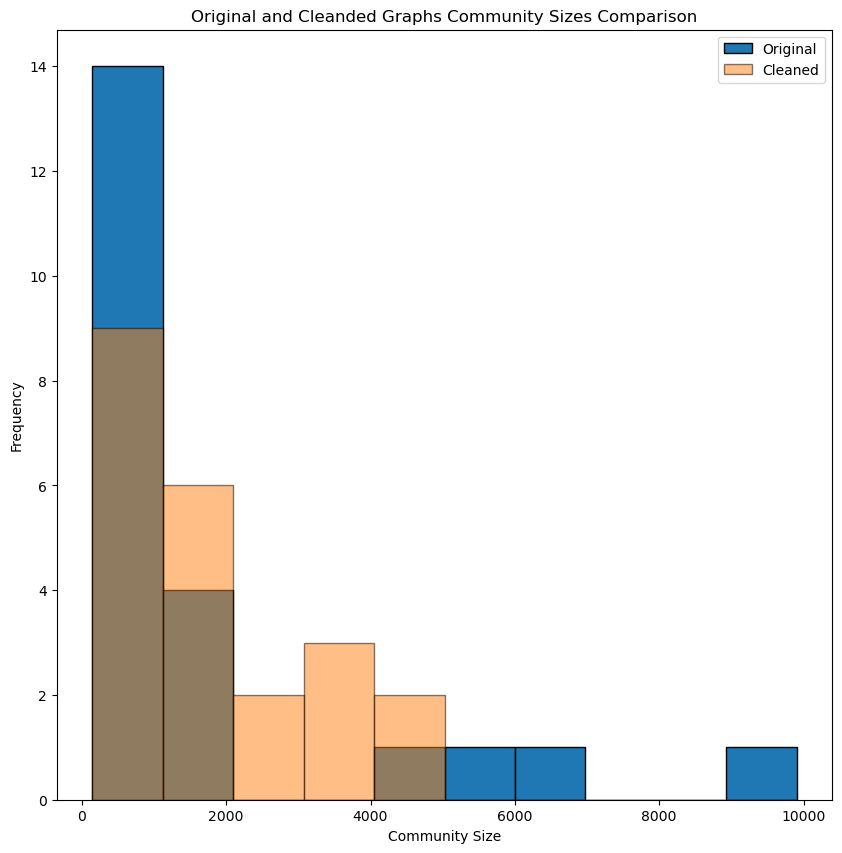
\includegraphics[width=0.45\textwidth]{images/Appendix_A/std_dv_community_sizes_comparison.png} \label{fig:std_dv_community_sizes_comparison} }
	\hfill \subfloat[Degree Centrality Distribution of Removed Nodes (Standard
	Deviation)]{%
	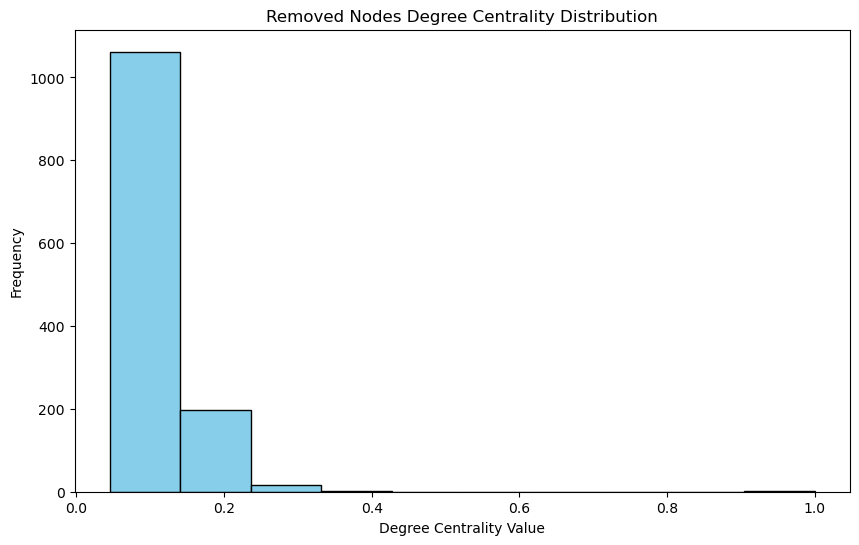
\includegraphics[width=0.45\textwidth]{images/Appendix_A/std_dv_removed_nodes_degree_centrality_distribution.png} \label{fig:std_dv_removed_nodes_degree_centrality_distribution} }
	\caption{Comparison of Community Sizes and Degree Centrality Distribution of
	Removed Nodes Using the Standard Deviation Method}
	\label{fig:std_dv_plots}
\end{figure}

\begin{figure}[h]
	\centering
	\subfloat[Community Sizes Comparison (Percentile)]{%
	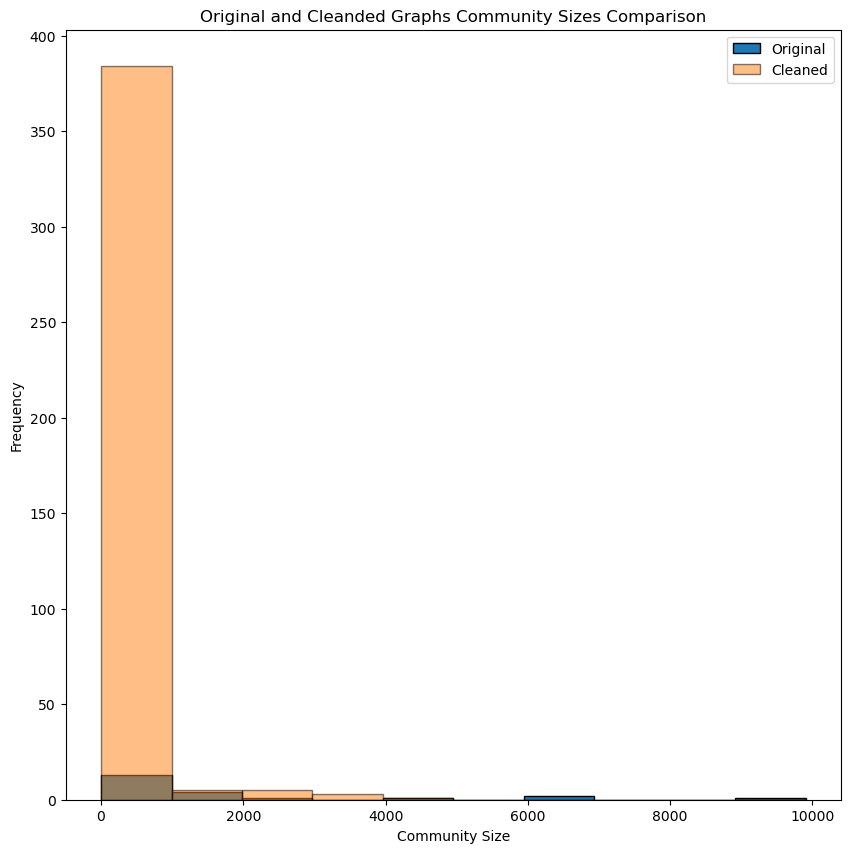
\includegraphics[width=0.45\textwidth]{images/Appendix_A/percentile_community_sizes_comparison.png} \label{fig:percentile_community_sizes_comparison} }
	\hfill \subfloat[Degree Centrality Distribution of Removed Nodes (Percentile)]{%
	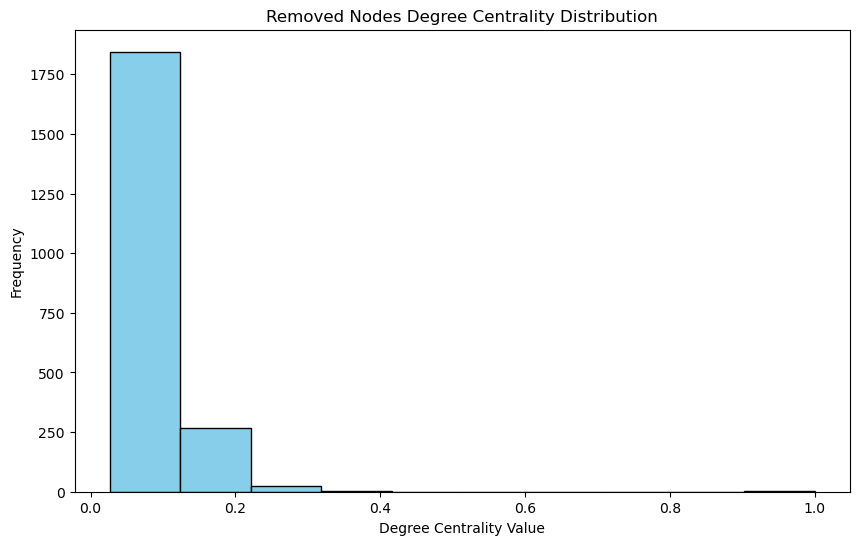
\includegraphics[width=0.45\textwidth]{images/Appendix_A/percentile_removed_nodes_degree_centrality_distribution.png} \label{fig:percentile_removed_nodes_degree_centrality_distribution} }
	\caption{Comparison of Community Sizes and Degree Centrality Distribution of
	Removed Nodes Using the Percentile Method}
	\label{fig:percentile_plots}
\end{figure}

\begin{figure}[h]
	\centering
	\subfloat[Community Sizes Comparison (IQR)]{%
	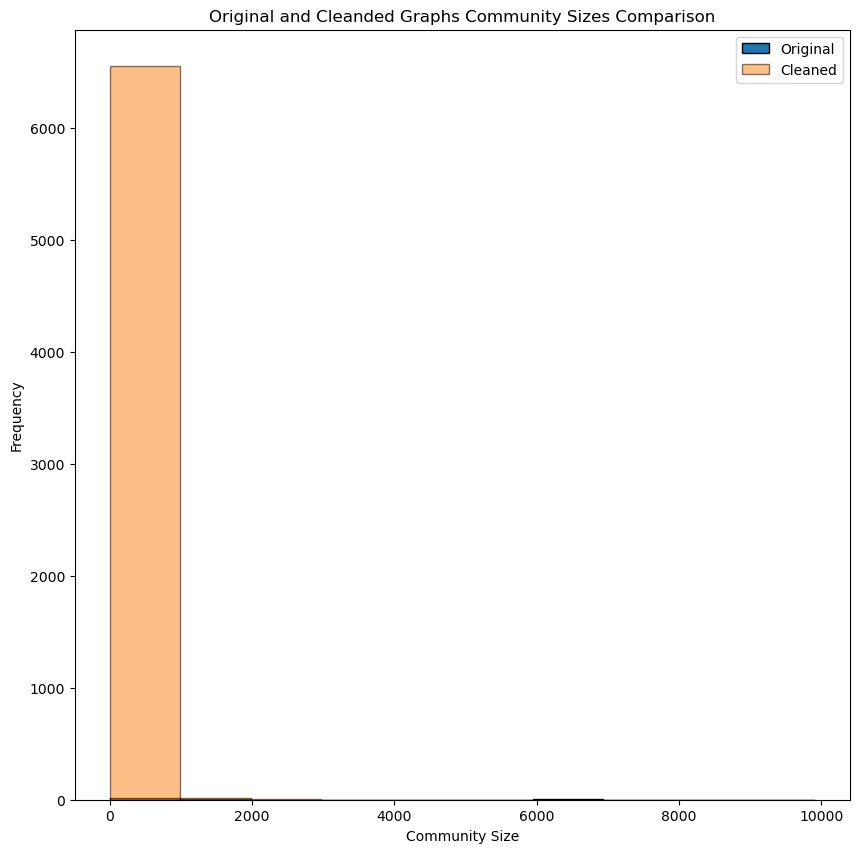
\includegraphics[width=0.45\textwidth]{images/Appendix_A/IQR_community_sizes_comparison.png} \label{fig:IQR_community_sizes_comparison} }
	\hfill \subfloat[Degree Centrality Distribution of Removed Nodes (IQR)]{%
	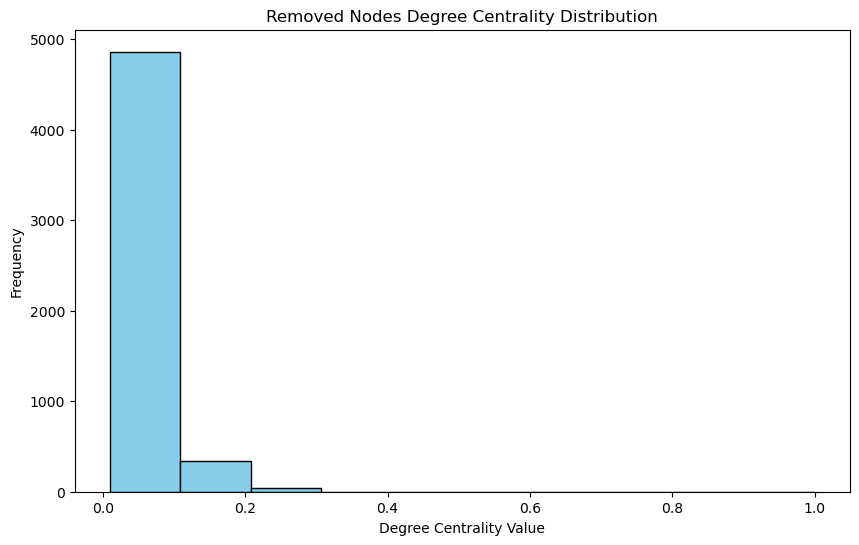
\includegraphics[width=0.45\textwidth]{images/Appendix_A/IQR_removed_nodes_degree_centrality_distribution.png} \label{fig:IQR_removed_nodes_degree_centrality_distribution} }
	\caption{Comparison of Community Sizes and Degree Centrality Distribution of
	Removed Nodes Using the IQR Method}
	\label{fig:IQR_plots}
\end{figure}

\begin{figure}[h]
	\centering
	\subfloat[Community Sizes Comparison (Knee Method)]{%
	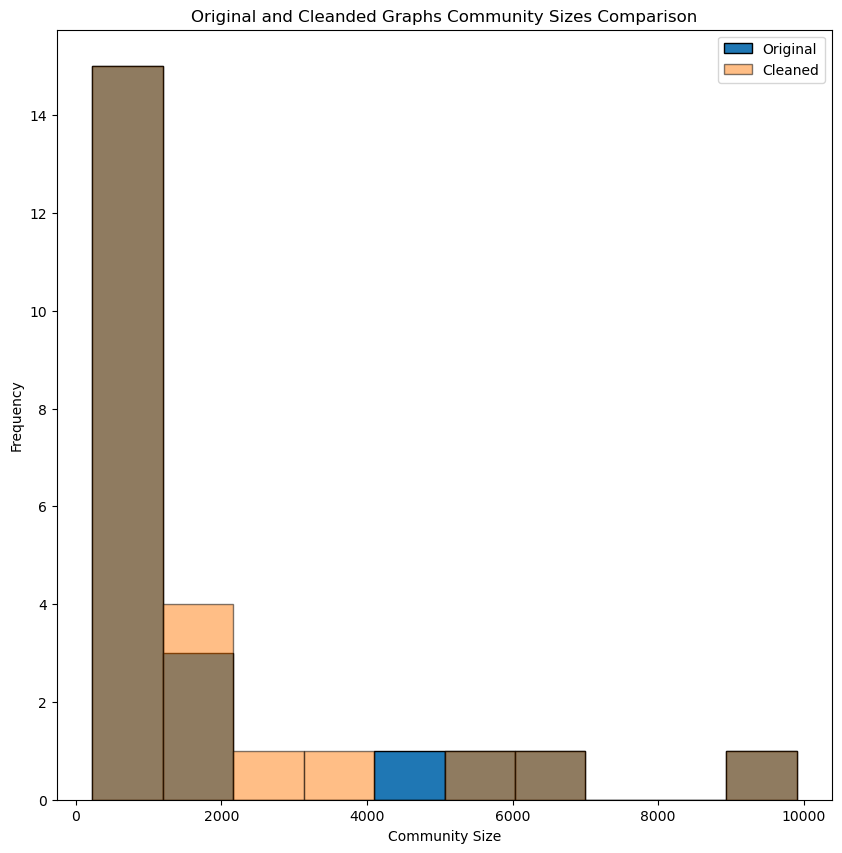
\includegraphics[width=0.45\textwidth]{images/Appendix_A/knee_community_sizes_comparison.png} \label{fig:knee_community_sizes_comparison} }
	\hfill \subfloat[Degree Centrality Distribution of Removed Nodes (Knee Method)]{%
	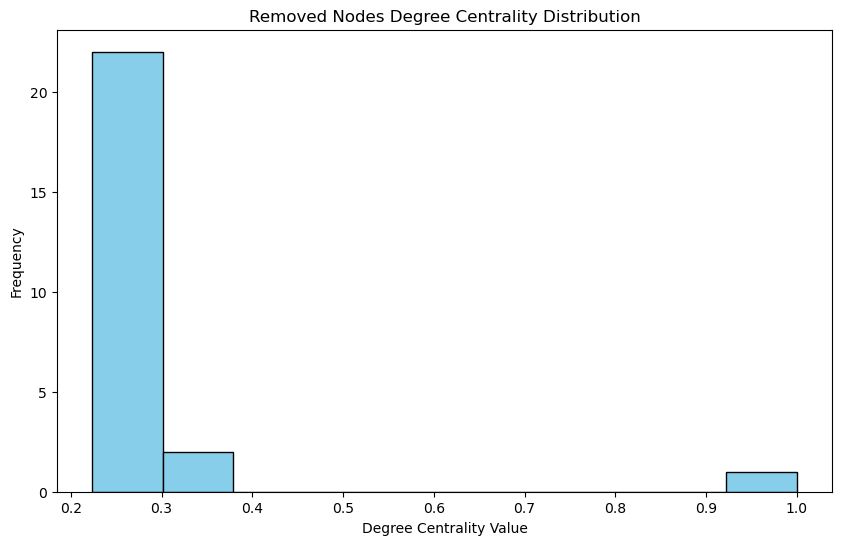
\includegraphics[width=0.45\textwidth]{images/Appendix_A/knee_removed_nodes_degree_centrality_distribution.png} \label{fig:knee_removed_nodes_degree_centrality_distribution} }
	\caption{Comparison of Community Sizes and Degree Centrality Distribution of
	Removed Nodes Using the Knee Method}
	\label{fig:knee_plots}
\end{figure}

\begin{figure}[h]
	\centering
	\subfloat[Community Sizes Comparison (Top 20 Method)]{%
	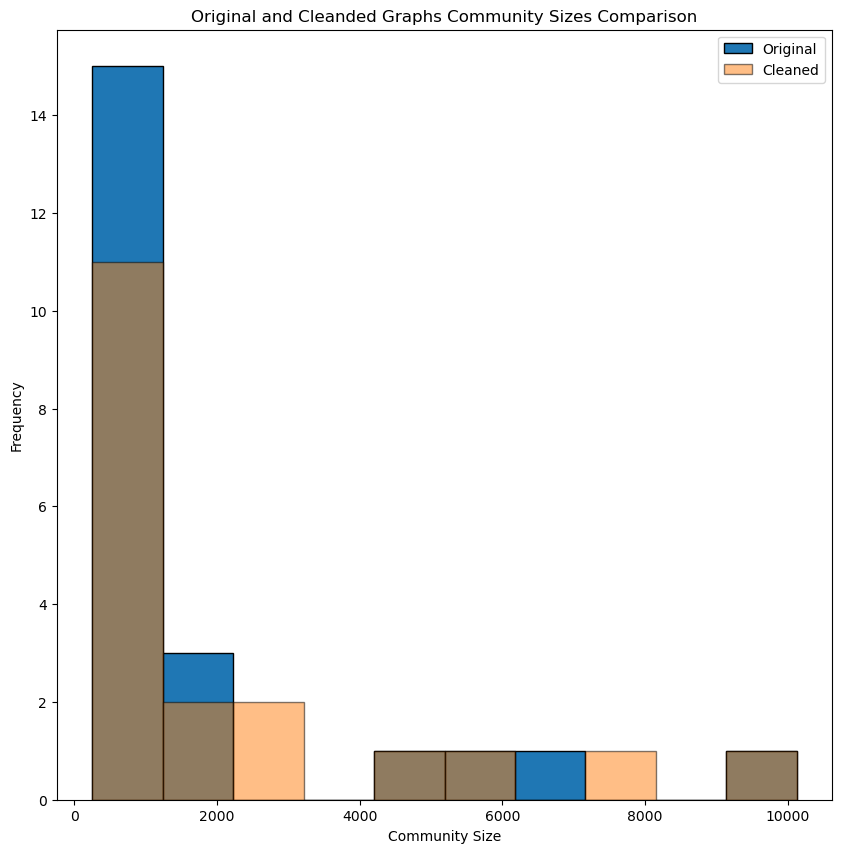
\includegraphics[width=0.45\textwidth]{images/Appendix_A/top20_community_sizes_comparison.png} \label{fig:top20_community_sizes_comparison} }
	\hfill \subfloat[Degree Centrality Distribution of Removed Nodes (Top 20
	Method)]{%
	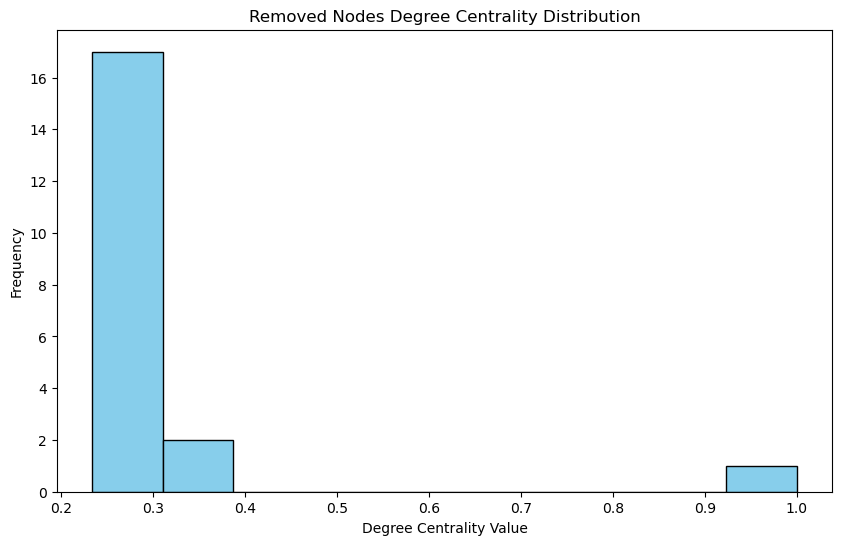
\includegraphics[width=0.45\textwidth]{images/Appendix_A/top20_removed_nodes_degree_centrality_distribution.png} \label{fig:top20_removed_nodes_degree_centrality_distribution} }
	\caption{Comparison of Community Sizes and Degree Centrality Distribution of
	Removed Nodes Using the Top 20 Method}
	\label{fig:top20_plots}
\end{figure}


\clearpage
\begin{table}[h]
	\centering
	\begin{adjustbox}
		{width=1.1\textwidth, center}
		\begin{tabular}{l c c c}
			\hline
			\textbf{Method/Metric} & \textbf{\# of Removed Nodes} & \textbf{\# Nodes in Cleaned Graph} & \textbf{\# of Communities in Cleaned Graph} \\
			\hline
			Standard Deviation     & 1279                         & 41391                              & 22                                          \\
			IQR                    & 5241                         & 37429                              & 6559                                        \\
			Percentile             & 2137                         & 40533                              & 398                                         \\
			Knee Method            & 25                           & 42645                              & 24                                          \\
			Top 20                 & 20                           & 42650                              & 19                                          \\
			\hline
		\end{tabular}
	\end{adjustbox}
	\caption{Comparison of Outlier Detection Methods}
	\label{tab:outlier_detection_methods}
\end{table} % Note, appendix must be last

\end{document}
